
\begin{figure}[htb]\begin{center}
	\subfigure[]{
  	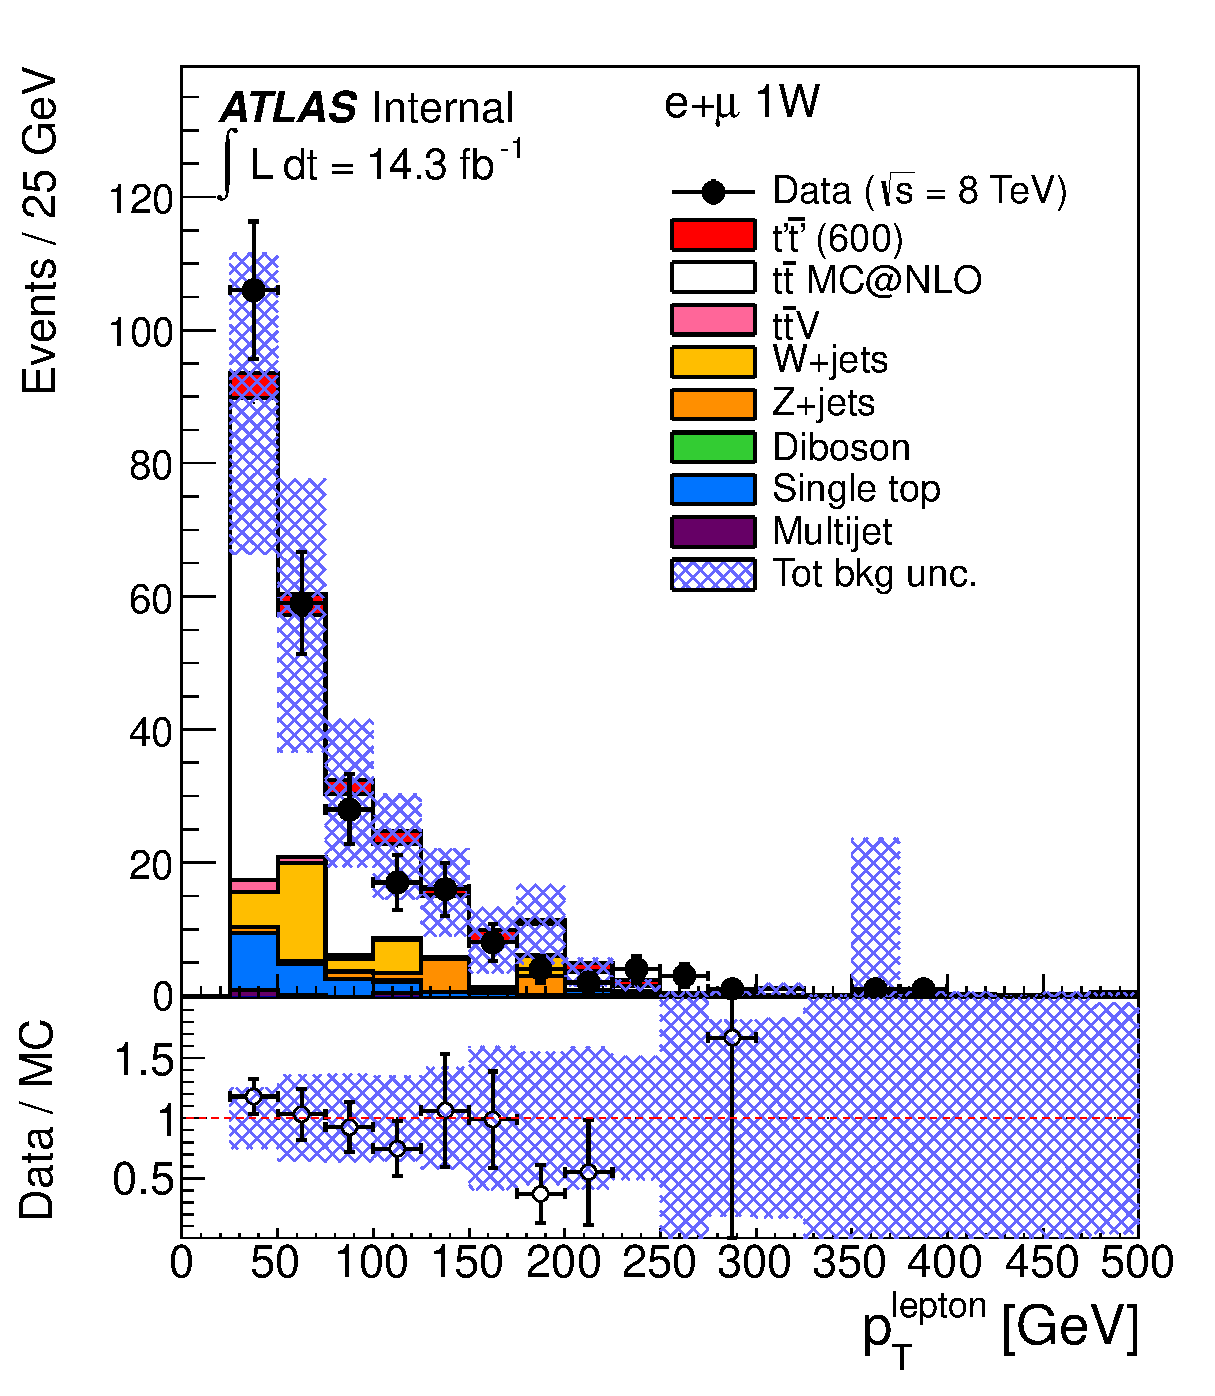
\includegraphics[width=0.31\textwidth]{appendices/figures/sdrs/LepPt_ELEMUONCR3_1W_NOMINAL}}
	\subfigure[]{
  	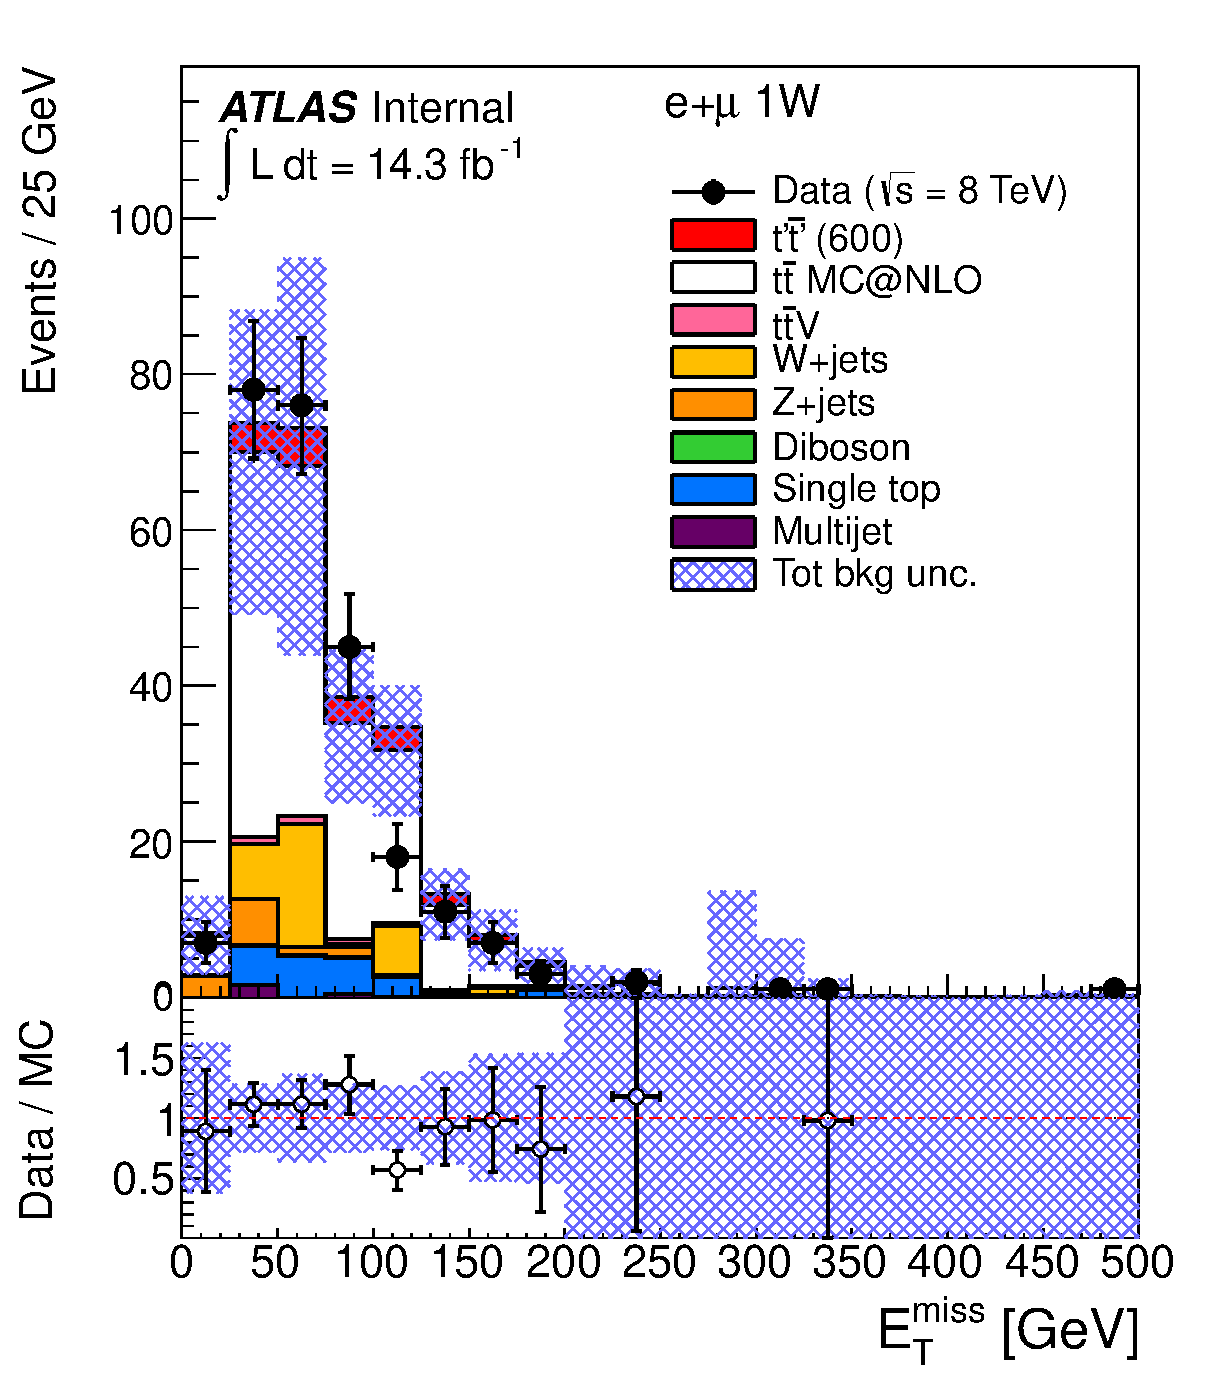
\includegraphics[width=0.31\textwidth]{appendices/figures/sdrs/MET_ELEMUONCR3_1W_NOMINAL}}
	\subfigure[]{
  	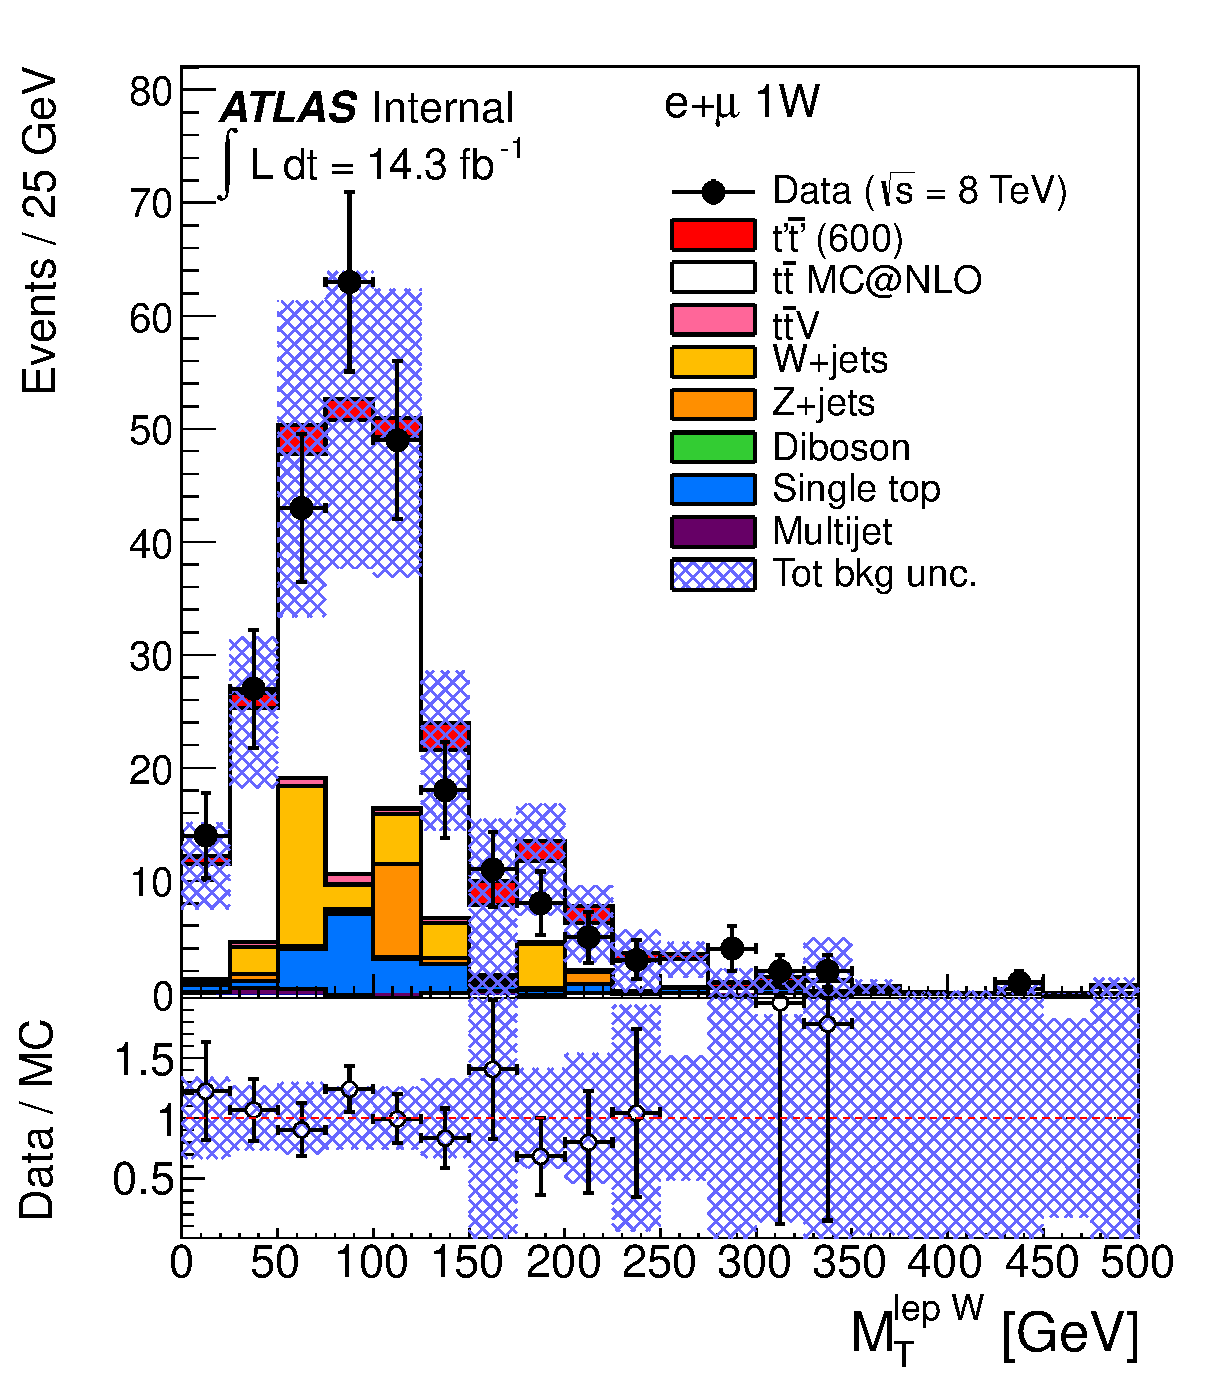
\includegraphics[width=0.31\textwidth]{appendices/figures/sdrs/Wlep_MassT_ELEMUONCR3_1W_NOMINAL}}
	\subfigure[]{
  	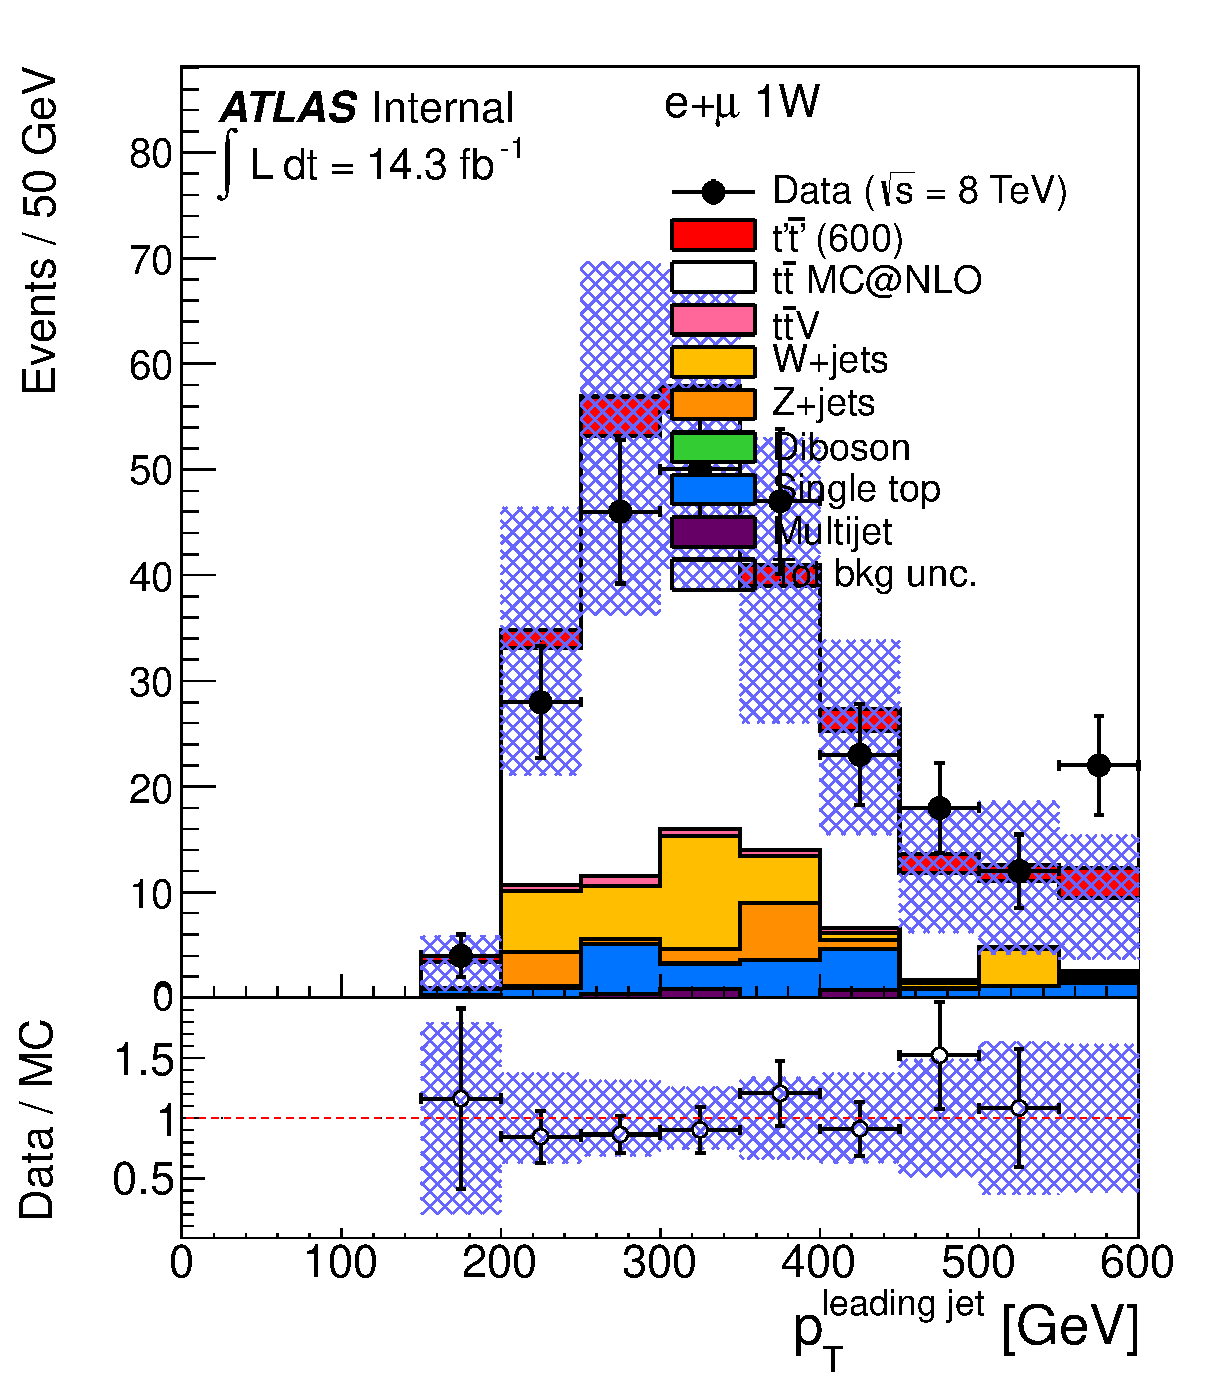
\includegraphics[width=0.31\textwidth]{appendices/figures/sdrs/JetPt1_ELEMUONCR3_1W_NOMINAL}}
	\subfigure[]{
  	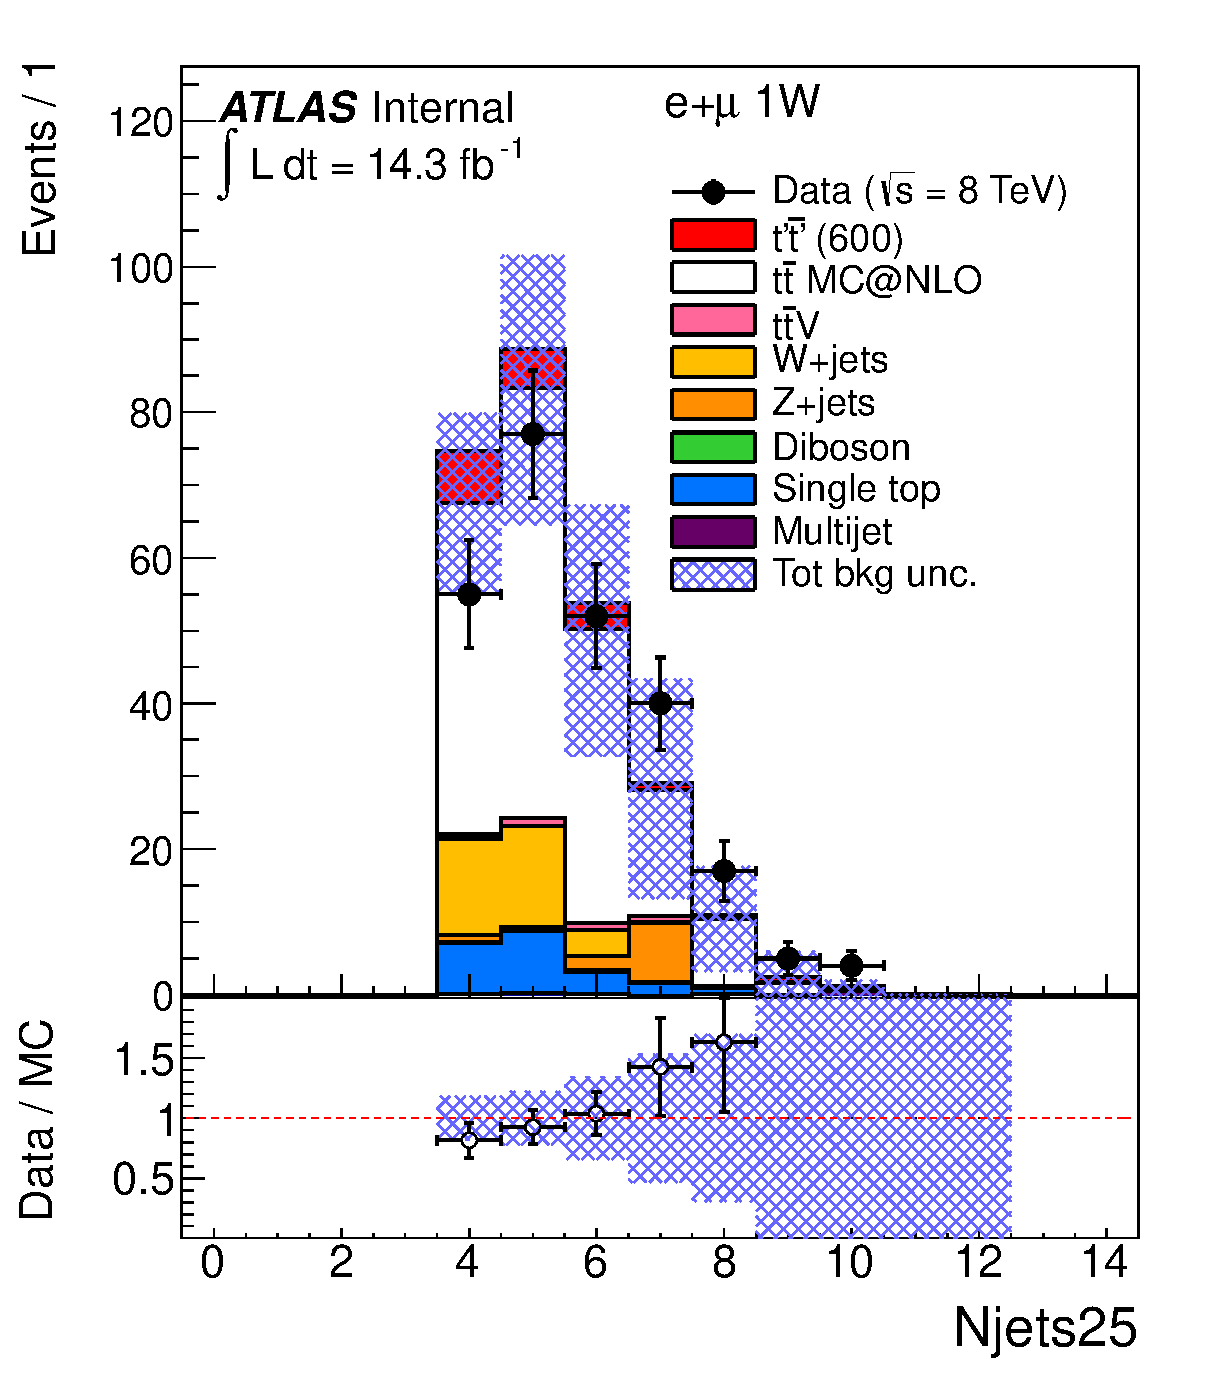
\includegraphics[width=0.31\textwidth]{appendices/figures/sdrs/Njets25_ELEMUONCR3_1W_NOMINAL}}
	\subfigure[]{
  	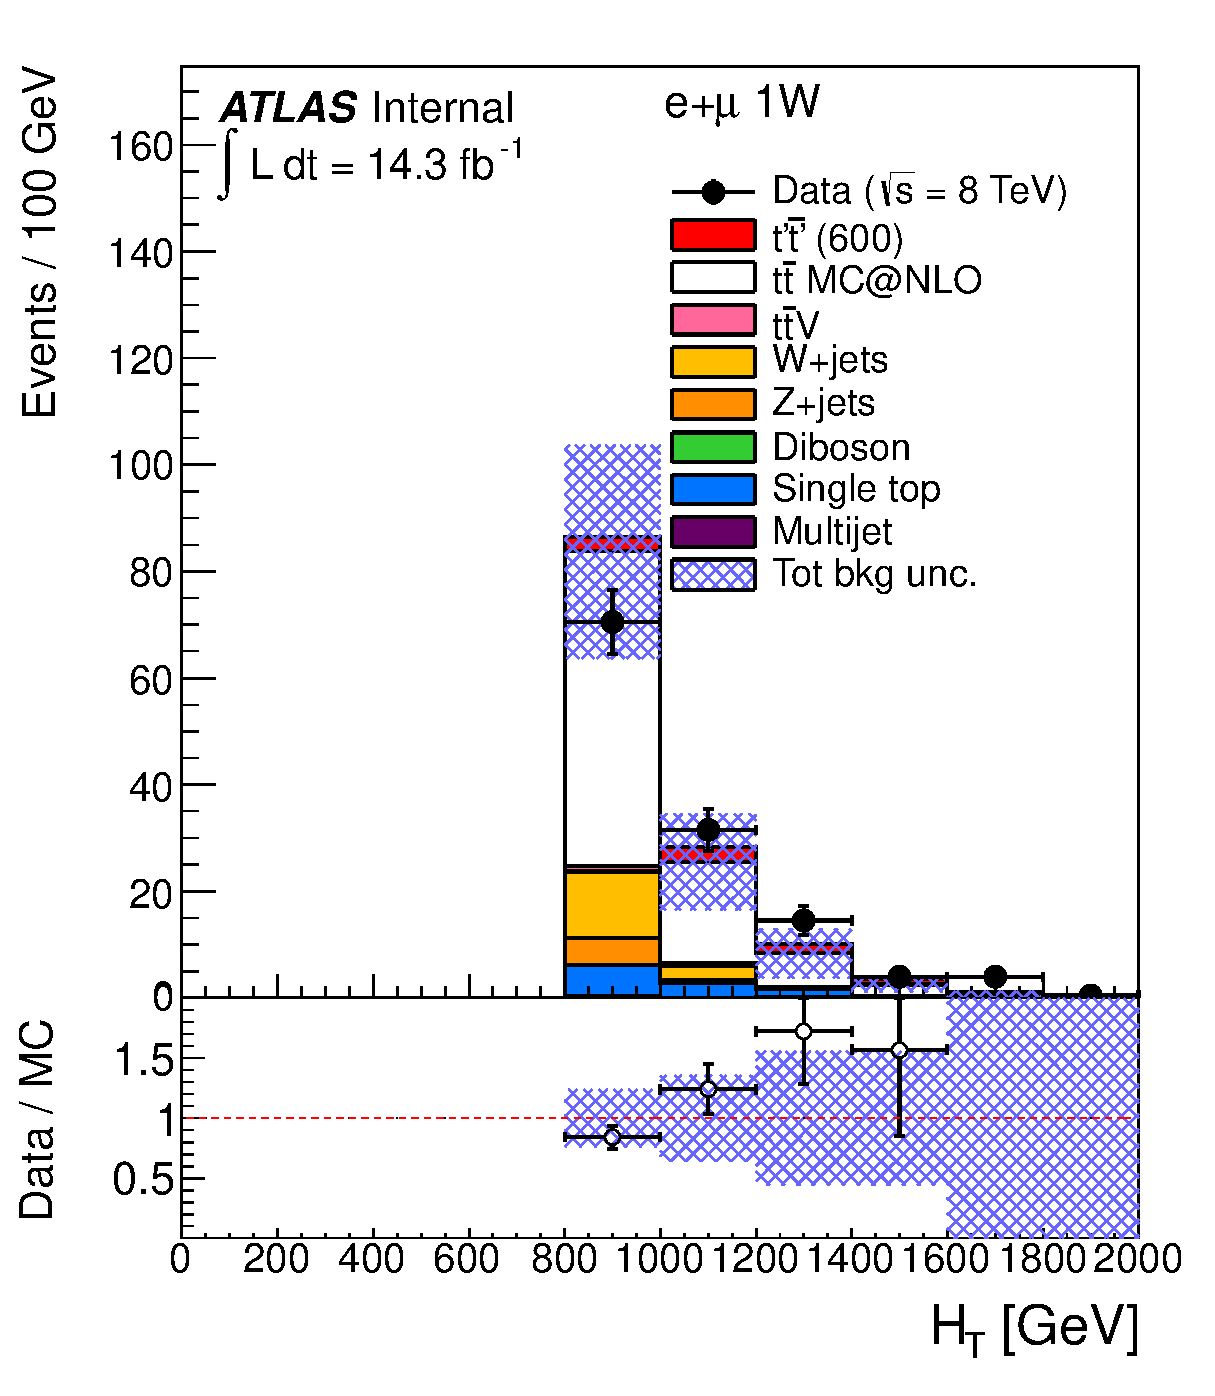
\includegraphics[width=0.31\textwidth]{appendices/figures/sdrs/HTAll_ELEMUONCR3_1W_NOMINAL}}
	\caption{Comparison between data and prediction plots for (a) lepton transverse momentum 
        (b) missing tranverse energy, (c) transverse mass of $W$ boson, (d)
        leading jet transverse momentum, (e) number of jets in the event with $\pt>25~\gev$,
        (f) $\HT$ variable in SDR4.
        The shaded area represents the total background uncertainty.\label{fig:sdr4}}
\end{center}\end{figure}

\begin{figure}[htb]\begin{center}
	\subfigure[]{
  	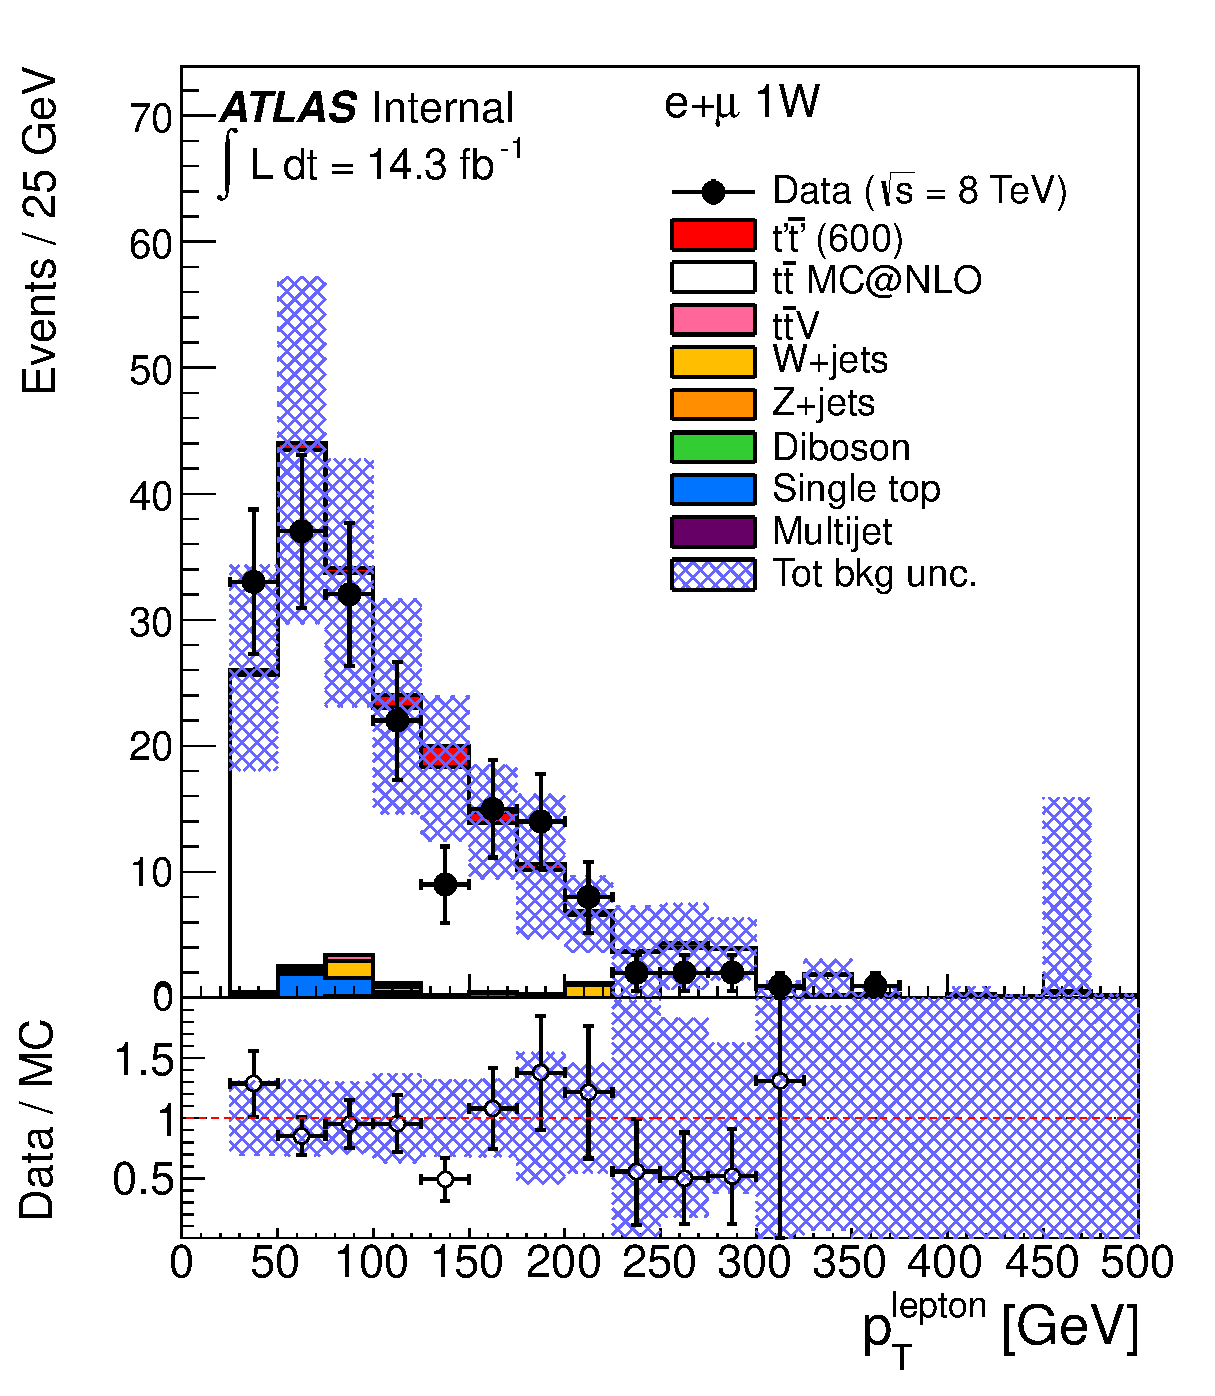
\includegraphics[width=0.31\textwidth]{appendices/figures/sdrs/LepPt_ELEMUONCR4_1W_NOMINAL}}
	\subfigure[]{
  	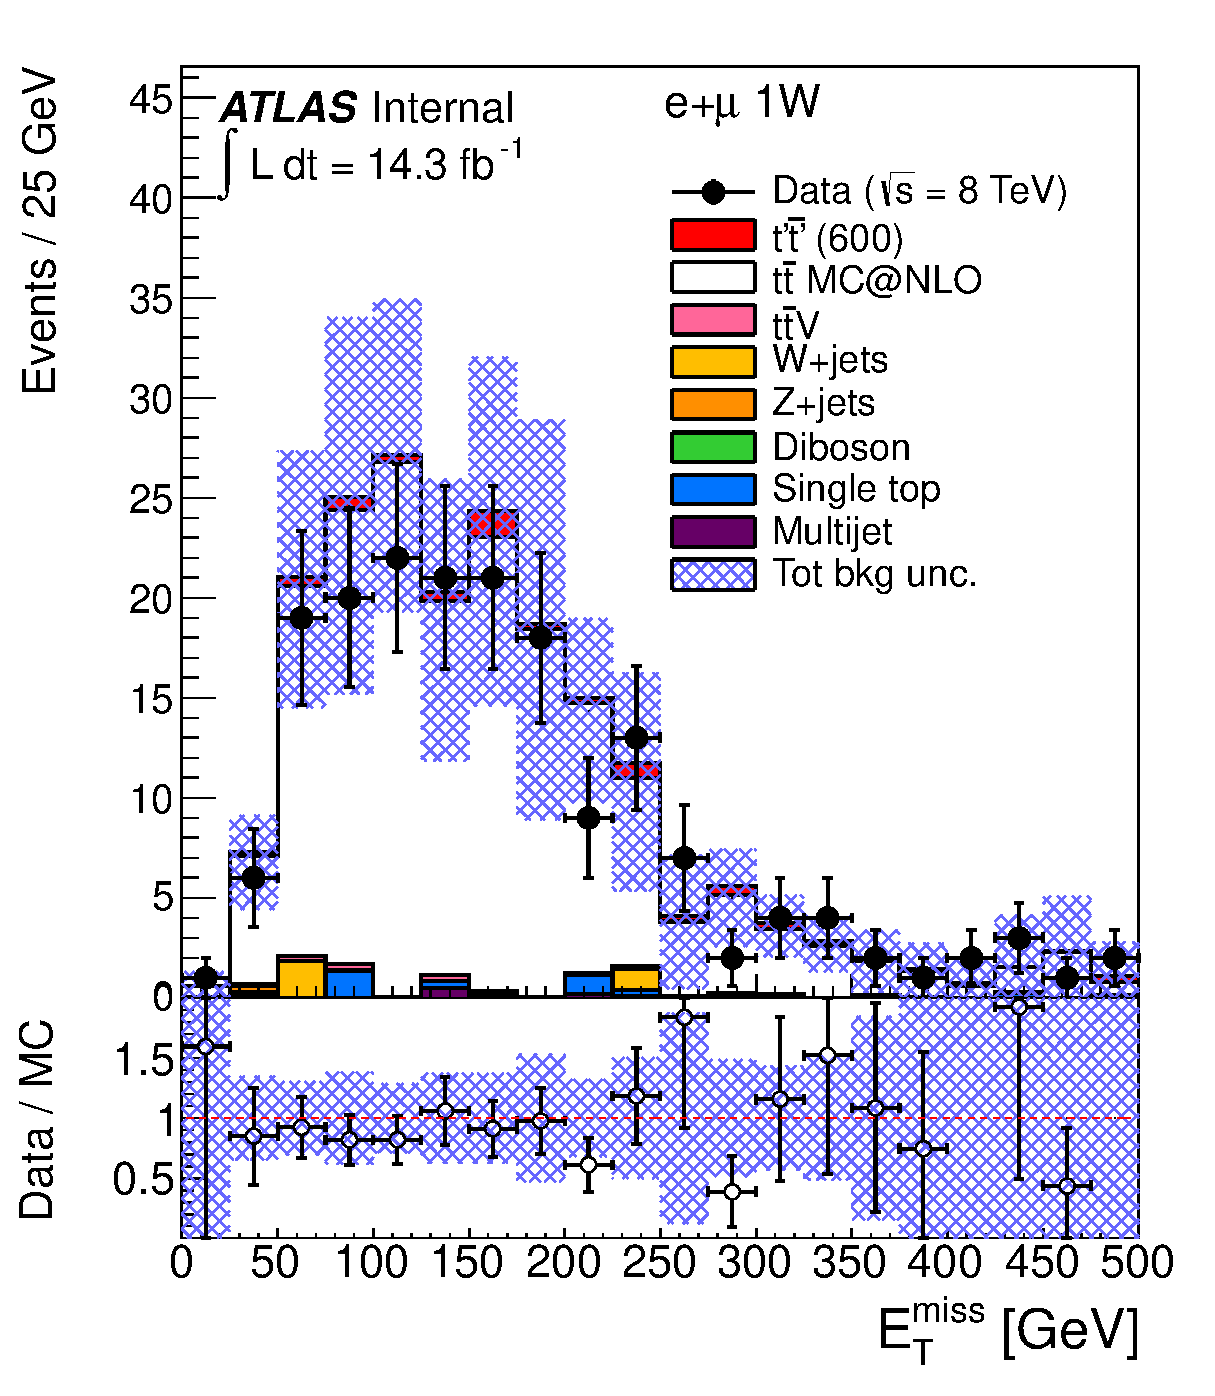
\includegraphics[width=0.31\textwidth]{appendices/figures/sdrs/MET_ELEMUONCR4_1W_NOMINAL}}
	\subfigure[]{
  	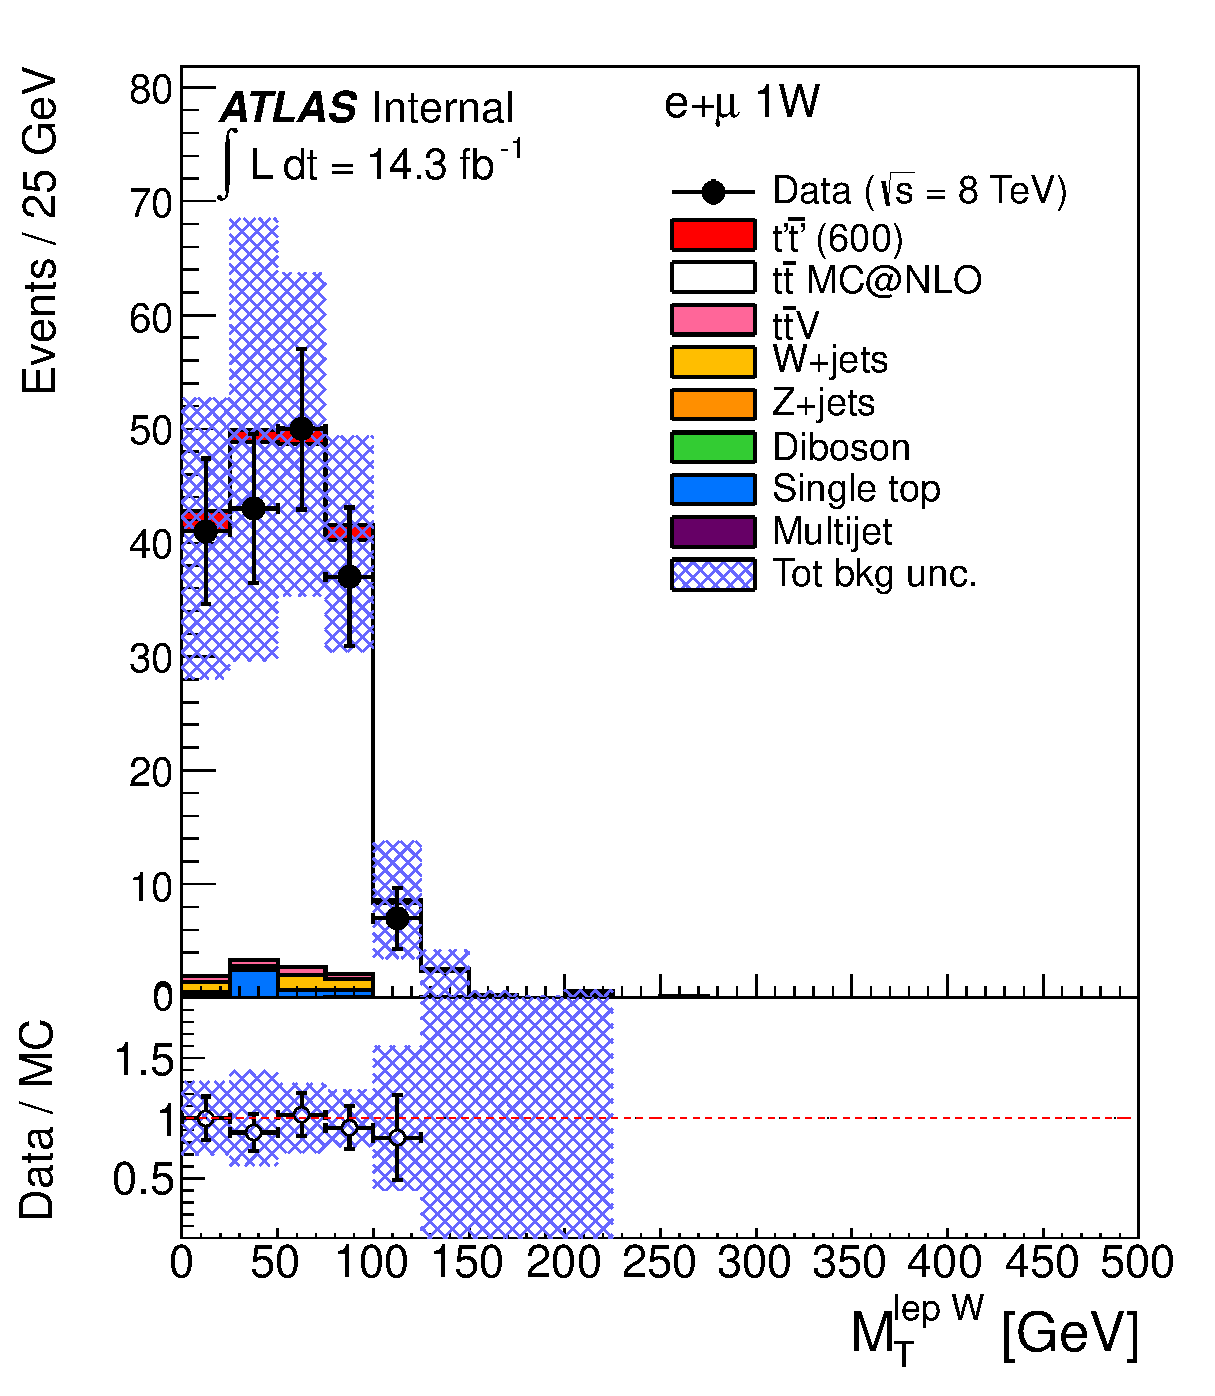
\includegraphics[width=0.31\textwidth]{appendices/figures/sdrs/Wlep_MassT_ELEMUONCR4_1W_NOMINAL}}
	\subfigure[]{
  	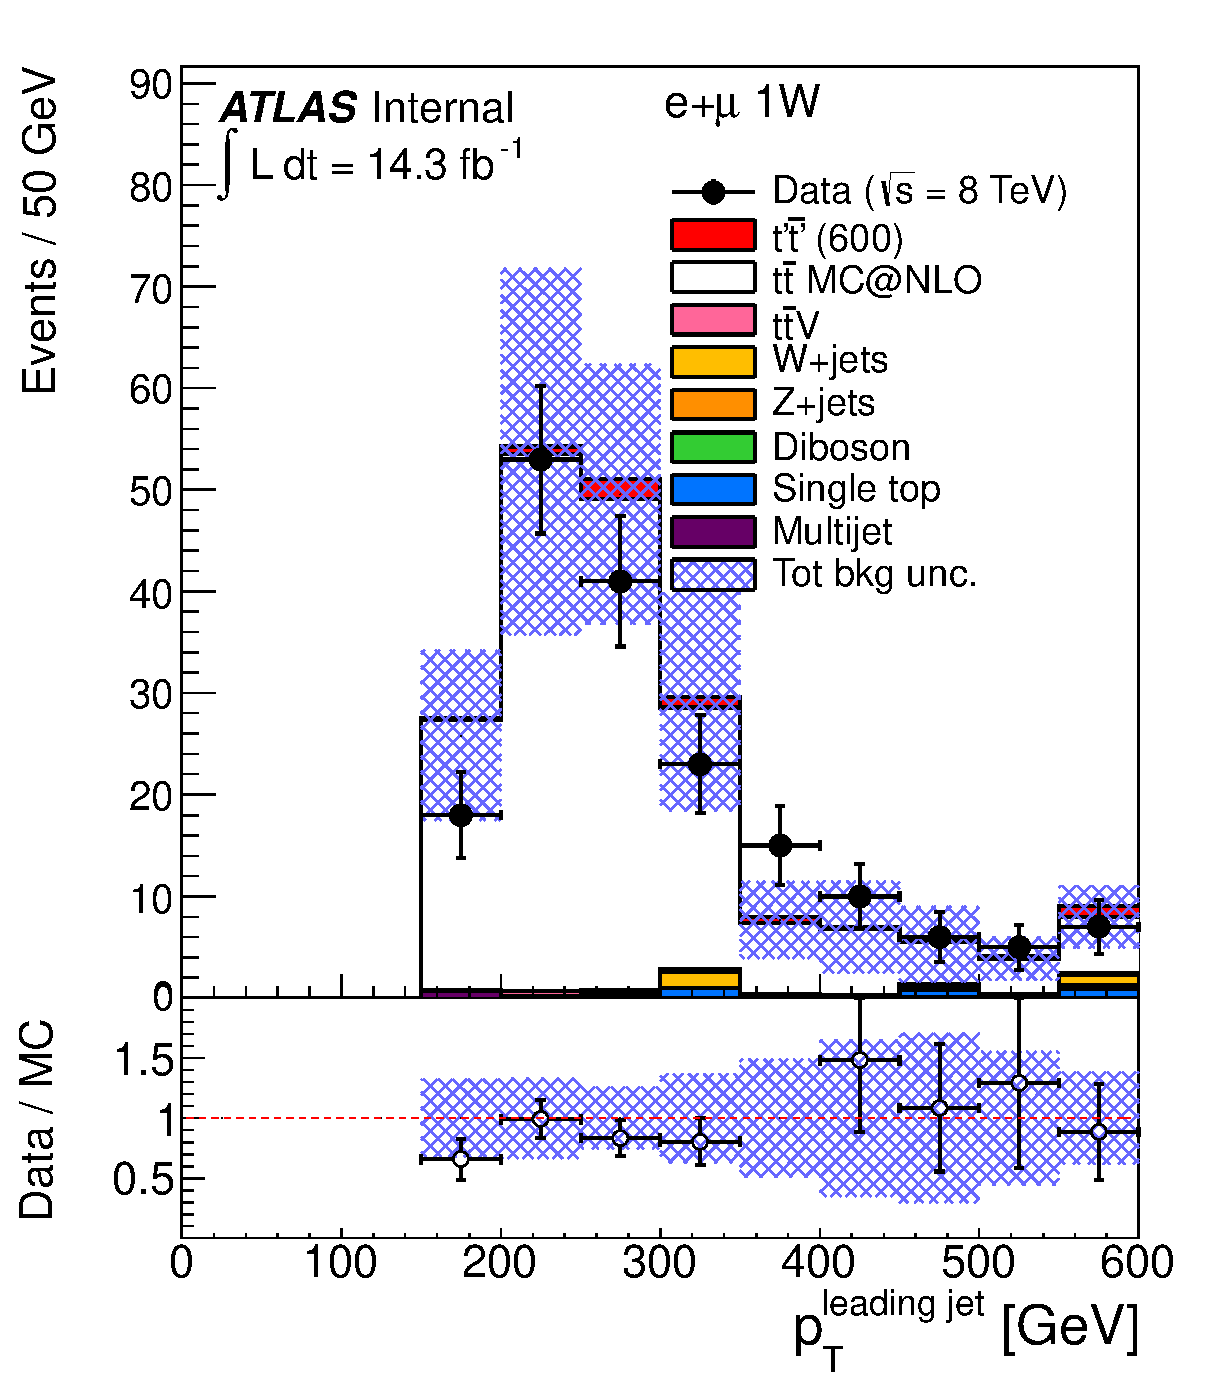
\includegraphics[width=0.31\textwidth]{appendices/figures/sdrs/JetPt1_ELEMUONCR4_1W_NOMINAL}}
	\subfigure[]{
  	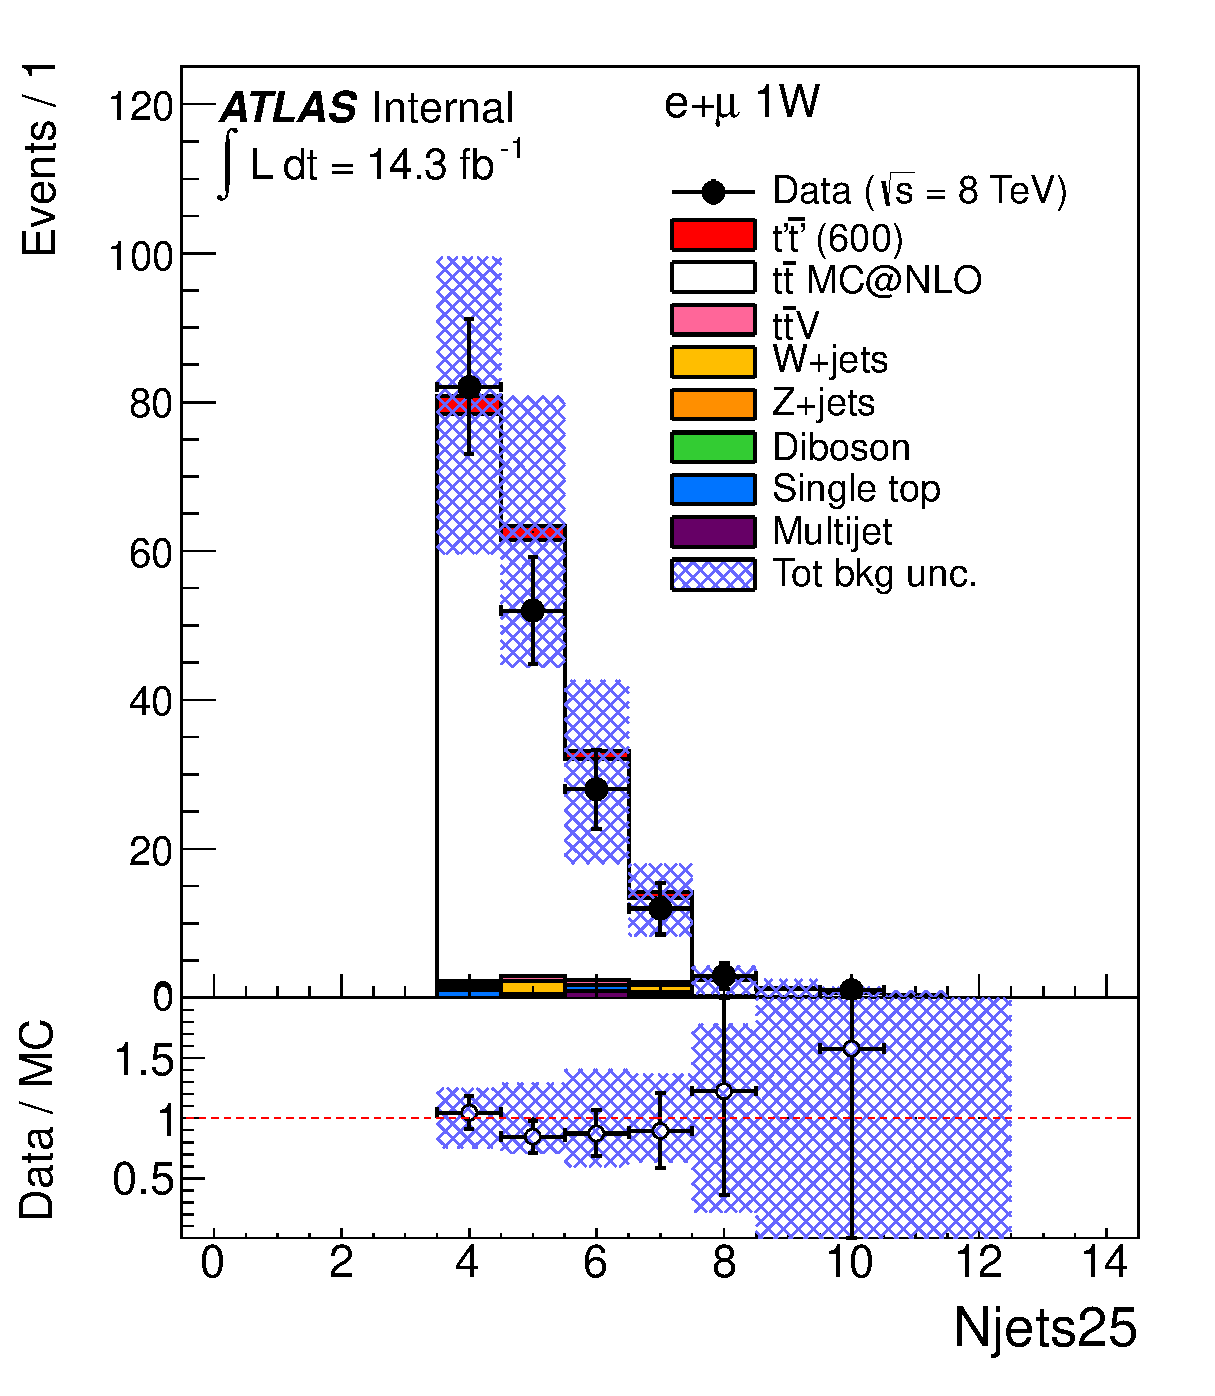
\includegraphics[width=0.31\textwidth]{appendices/figures/sdrs/Njets25_ELEMUONCR4_1W_NOMINAL}}
	\subfigure[]{
  	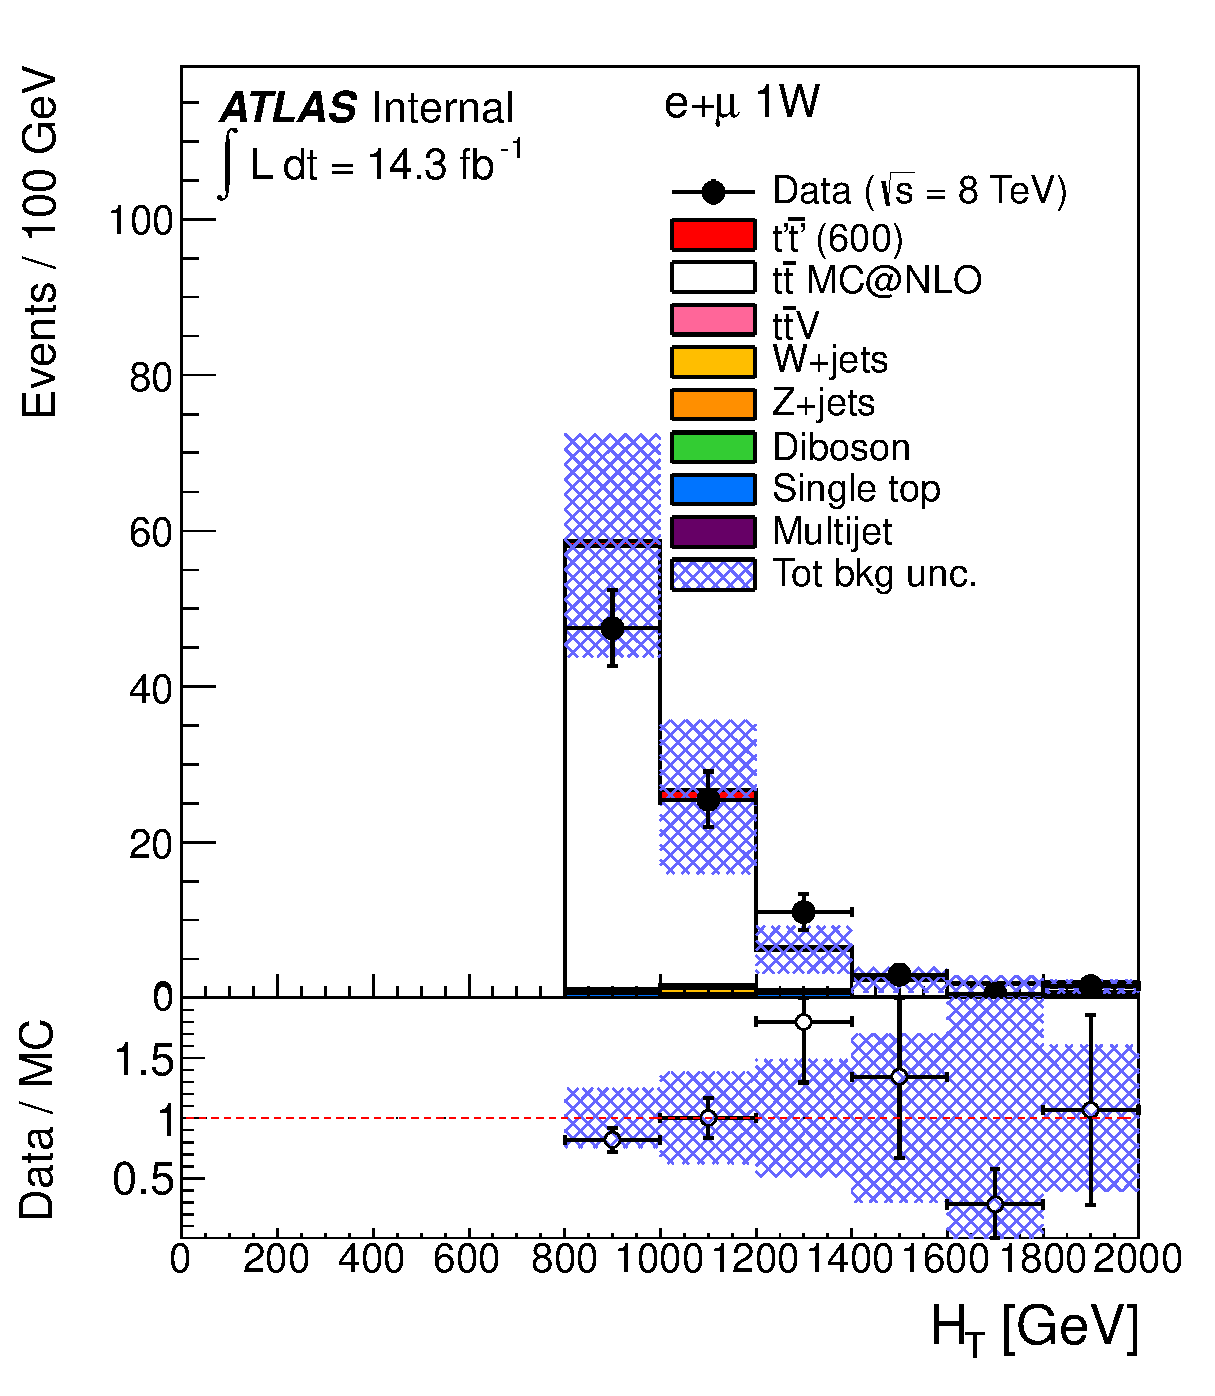
\includegraphics[width=0.31\textwidth]{appendices/figures/sdrs/HTAll_ELEMUONCR4_1W_NOMINAL}}
	\caption{Comparison between data and prediction plots for (a) lepton transverse momentum 
        (b) missing tranverse energy, (c) transverse mass of $W$ boson, (d)
        leading jet transverse momentum, (e) number of jets in the event with $\pt>25~\gev$,
        (f) $\HT$ variable in SDR5.
        The shaded area represents the total background uncertainty.\label{fig:sdr5}}
\end{center}\end{figure}
